\documentclass{article}
\usepackage{xstring}
\usepackage{tikz}
\usetikzlibrary{calc}

%    Column B contains numbers 1 - 15
%    Column I contains numbers 16 - 30
%    Column N contains numbers 31 - 45
%    Column G contains numbers 46 - 60
%    Column O contains numbers 61 - 75

\def\NumOfColumns{5}%
\def\Sequence{1/A/1/15, 2/B/16/30, 3/C/31/45, 4/D/46/60, 5/E/61/71}%

\newcommand{\Size}{2.5cm}
\tikzset{Square/.style={
    inner sep=0pt,
    text width=\Size, 
    minimum size=\Size,
    draw=black,
    fill=yellow!20,
    align=center,
    }
}

\begin{document}
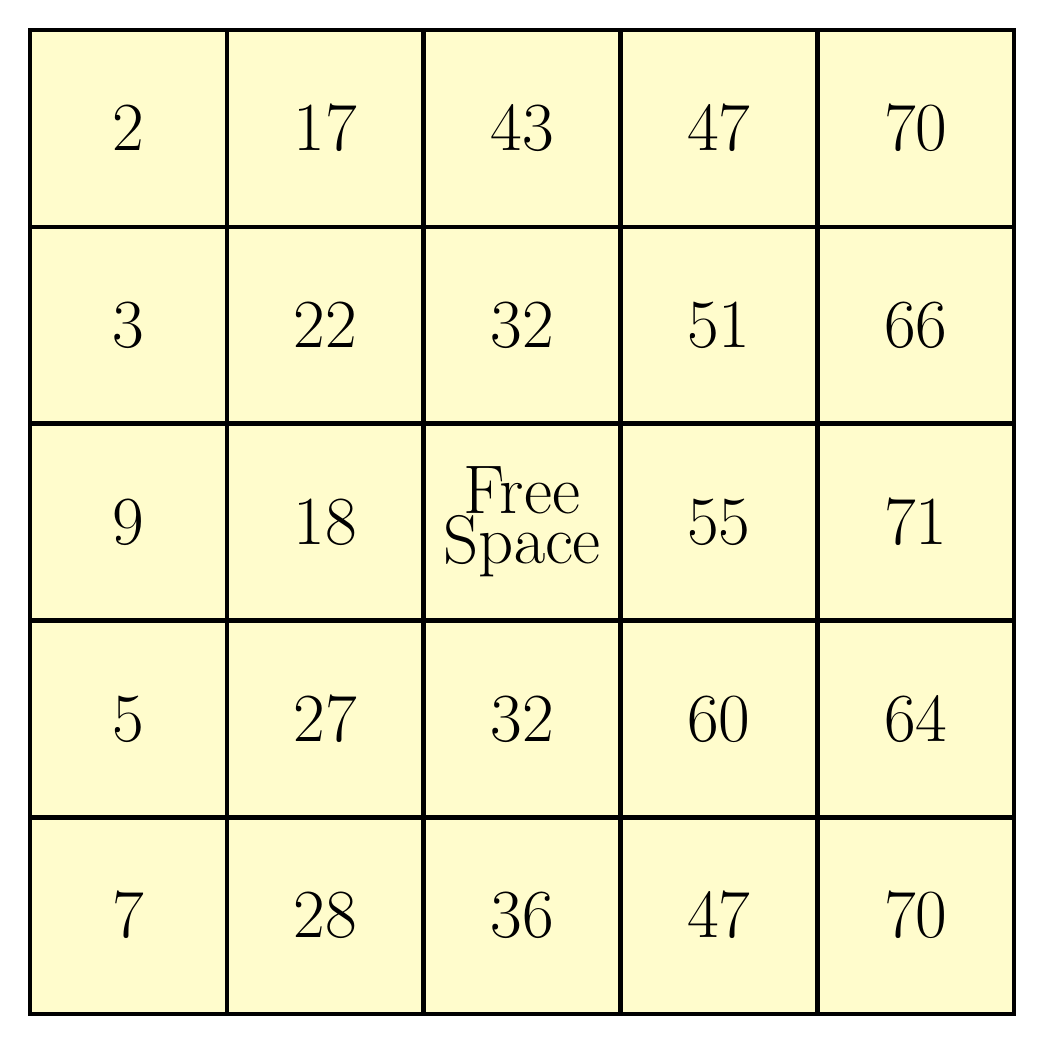
\begin{tikzpicture}[draw=black, ultra thick, x=\Size,y=\Size]
    \foreach \row/\rowLetter/\MinNumber/\MaxNumber in \Sequence{%
        \foreach \col/\colLetter/\MinNumber/\MaxNumber in \Sequence {%
            \pgfmathtruncatemacro{\value}{\col+\NumOfColumns*(\row-1)}
            \def\NodeText{\pgfmathparse{random(\MinNumber,\MaxNumber)}\pgfmathresult}
            \pgfmathsetmacro{\ColRowProduce}{\col*\row}
            \IfEq{\ColRowProduce}{9}{% If is center square
                \node [Square] at ($(\col,-\row)-(0.5,0.5)$) {\Huge Free Space};
            }{
                \node [Square] at ($(\col,-\row)-(0.5,0.5)$) {\Huge \NodeText};
            }
        }
    }
\end{tikzpicture}
\end{document}